\documentclass[12pt,a4paper]{article}
\usepackage[utf8]{inputenc}
\usepackage{amsmath}
\usepackage{amsfonts}
\usepackage{amssymb}
\usepackage{color}
\author{Zhuoran Liu}
\title{Multi-Layer Perceptron}
\usepackage{graphicx}

\begin{document}
\maketitle

\color{black}
\newpage
\section{Introduction}
In this report, we will consider the neural network multi-layer perceptron. Multi-layer perceptron is a neural network with multiple hidden layers and in each hidden layer there are multiple neurons. Between different neurons in adjacent layers, there exist weights to connect different neurons. In every hidden layer, there exist biases to tune some outcomes of neurons. The aim of training the network is to find the proper weights and biases which can be used to predict the new data.
\subsection{Underlying Theory}
Firstly, we will talk about the working mechanism of the MLP. Given the neural network structure(weights matrix $W$ and biases vector $b$) and input data vector $a$, we can calculate the feed forward process by formula
\[\textbf{z} = g(\textbf{w}a + \textbf{b})\]
Here $g$ is the activation function and output $z$ is a vector. Use $z$ as the input of the next layer, we can do similar calculation again until we get the output. Given the last output $z$, we will calculate the $argmax(z)$. The category of the $argmax(z)$ is the predication of the input $a$. Known the right category, we will tune the weights and biases to predict better and better. This is the learning process of MLP. 
Given the input 
\subsection{Learning Algorithm}
Backpropagation algorithm is the learning algorithm we will use. It consists of 4 steps.
\[\delta^L = \nabla_{a} C \circ \sigma'(z^{L})\]
\[\delta^L = ((w^{l+1})^{T} \delta^{l+1} \circ \sigma'(z^{l})\]
\[\frac{\partial C}{\partial b_{j}^{l}} = \sigma_{j}^{l}\]
\[\frac{\partial C}{\partial w_{jk}^{l}} = a_{k}^{l-1} \sigma_{j}^{l}\]
This four step will backpropagate error and output the gradient change of cost function. The whole process is input, feedforward, backpropagate, update weights and biases, input again... Finally after many epoches we will get the final neural network with particular weights and biases, then we finish training.
\newpage
\section{Problem statement}
1. The influence of different layers and different number of neurons.\\
2. The different initializations of the weights and biases before learning.\\
3. Different chooses of activation functions.\\
4. different learning method Stochastic Gradient Descent vs. Momentum.\\
\section{Results}
\subsection{The structure of Multi-Layer Perceptron}
\subsubsection{Different neurons}
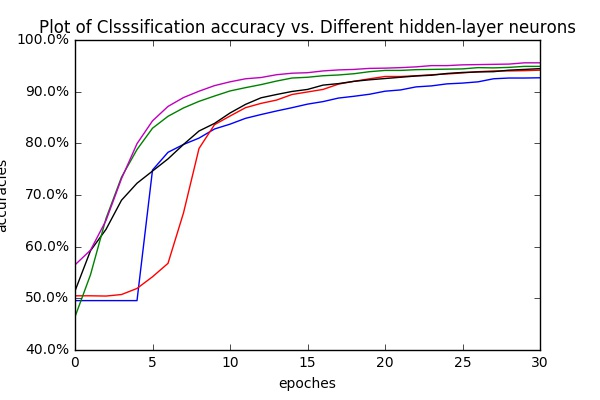
\includegraphics[width=90mm,scale=1]{p101.jpg}\\
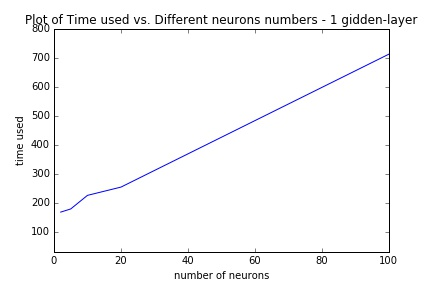
\includegraphics[width=90mm,scale=1]{p102.jpg}\\
\subsubsection{Different layers}
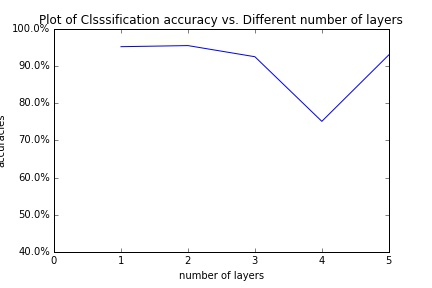
\includegraphics[width=90mm,scale=1]{p103.jpg}\\
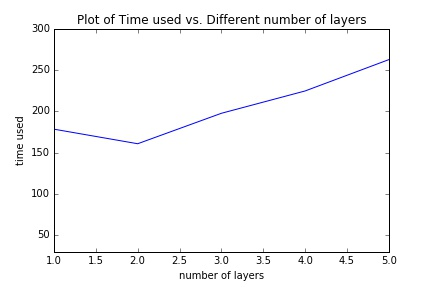
\includegraphics[width=90mm,scale=1]{p104.jpg}\\
\subsection{The initialization of the weights and biases}

\subsubsection{different initialization of weights and biases}
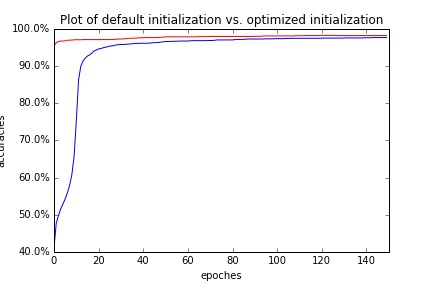
\includegraphics[width=90mm,scale=1]{p201.jpg}\\

\subsubsection{different activation functions}
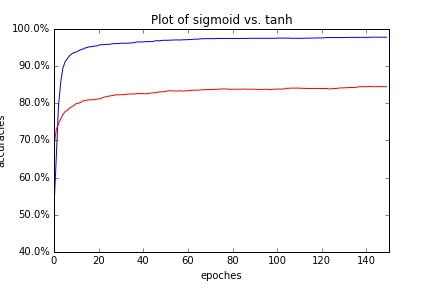
\includegraphics[width=90mm,scale=1]{p301.jpg}\\


\subsection{Different learning methods}
\subsubsection{Stochastic gradient descent}
\subsubsection{Momentum learning}


\section{Discussion}


\section{Conclusion}


\newpage
\section{Appendix}
\end{document}